
\subsection{Simulation Framework} \label{sec:architecture}

We assume that Alice and Bob have already established an authenticated classical communication channel. The BB84 quantum key distribution (QKD) protocol consists of a quantum preparation–measurement phase followed by a classical post-processing phase. In this subsection, we describe how a Qiskit program is constructed to simulate the first phase, combining Alice’s qubit preparation and Bob’s measurements of the transmitted qubits within a single quantum circuit. Eve’s eavesdropping is also incorporated into this circuit.

Our Qiskit program is executed in a hybrid environment: locally and on IBM’s quantum platforms. To run the circuit on IBM hardware, we installed IBM Qiskit Runtime, created an IBM Cloud account, and obtained an access token for the simulation. 
IBM provides limited free access to its quantum processing units (QPUs), with a cap of 10 minutes of execution time per month on devices with over 100 qubits. 
Given these resource constraints, we restrict our implementation of BB84 QKD to 20 qubits for Alice and Bob. 
We also note that Qiskit is unable to simulate BB84 circuits with 25 or more qubits, due to the exponential growth of the Hilbert space, which reaches dimension $2^N$ where $N$ is the number of qubits.

While our implementation follows IBM’s BB84 QKD framework \cite{IBM_QKD_website}, we have refactored the code into modular helper functions to improve clarity and reusability. 
In addition, we also added the key classical post-processing steps: error correction and privacy amplification.

The core components are outlined below:

(a) To implement Alice’s encoding, we define the helper function encode\_bb84\_states, which specifies how Alice prepares her qubits based on her randomly generated bit string and randomly chosen bases. Figure \ref{fig:encoding} illustrates this publicly known encoding scheme.

\begin{figure}[htbp]
\centering
\centerline{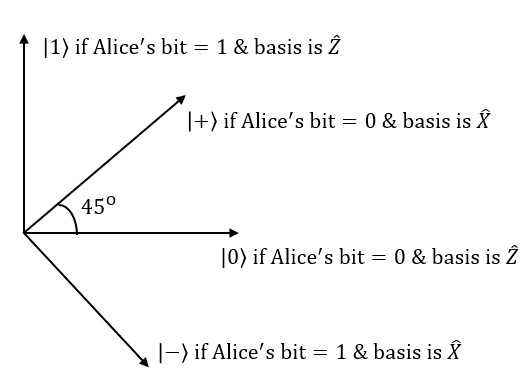
\includegraphics[scale=0.7]{Figures/encoding.jpg}}
\caption{Bit-to-Qbit encoding based on Alice's basis}
\label{fig:encoding}
\end{figure}

(b) To implement Bob’s measurements of Alice’s qubits, we define two helper functions: measure\_bb84 and counts\_to\_bbits. The first models Bob’s measurement outcomes based on his randomly chosen bases, while the second converts these outcomes into classical bits according to the encoding scheme.

(c) To construct Alice and Bob's sifted keys, we define the helper function sift\_key, which compares their basis choices and retains only the bits for which the bases coincide. In practice, Alice and Bob exchange their basis choices over the authenticated classical channel; this exchange is not explicitly simulated here.

(d) To compute the quantum bit error rate (QBER), we define the helper function key\_statistics, which compares Alice’s and Bob’s sifted keys and calculates the fraction of differing bits. In the ideal case without noise, QBER should be zero.

(e) To simulate the BB84 QKD protocol in the absence of an eavesdropper, we define the helper function simulate\_BB84. This function accepts a noise model as input, allowing execution either locally or on an IBM quantum platform.

(f) To simulate Eve’s intercept-and-resend attack, we define the helper function eavesdropper\_experiment. In this routine, Eve intercepts each qubit sent by Alice, measures it using a randomly chosen basis, records the outcome, and forwards the resulting state to Bob.

(g) To correct errors in Bob's sifted key, we define two key helper functions: locate\_and\_fix\_error and cascade\_protocol. The latter implements the Cascade protocol that corrects errors based on a backtracking procedure on multiple blocks of Bob's sifted key. 
The former is used within the latter to find and correct each incorrect bit.

(h) To implement privacy amplification, we define the helper function generate\_toeplitz, which constructs a random binary Toeplitz matrix. This matrix is used to map the original key to a shorter one, effectively diffusing any information across the resulting key.